\documentclass[25pt, a0paper, landscape, cmyk]{tikzposter}
% Fontspec changes the metrics slightly (!)
%\usepackage{fontspec}%\setsansfont{Montserrat Black}
% Use a simpler package instead
\input font-change-xetex
\mysanzfont{Montserrat Black}{28}{letterspace=6}
\usepackage[colorlinks,allcolors=blue]{hyperref}
\tikzposterlatexaffectionproofoff
\title{Edit Conflicts, Offline Contributions, and Tor: Oh My!}
\author{%
  C. Scott Ananian %\texttt{[[User:cscott]]}
  <cananian@wikimedia.org> and
  Arlo Breault %\texttt{[[User:Arlolra]]}
  <abreault@wikimedia.org>,
  Wikimedia Foundation
}
\definecolorpalette{Wikimania2018}{
  % Red: 213 0 0 = D50000
  % Yellow: 255 193 7 = FFC107
  % Green: 0 174 66 = 00AE42
  \definecolor{colorOne}{HTML}{000000} % Black
  \definecolor{colorTwo}{HTML}{00AE42} % Green
  \definecolor{colorThree}{HTML}{D50000} % Red
  \definecolor{colorFour}{HTML}{FFC107} % Yellow
}
\definecolorstyle{CapeTown}{
  \definecolor{colorOne}{HTML}{FFC107}
  \definecolor{colorTwo}{HTML}{00AE42}
  \definecolor{colorThree}{HTML}{D50000}
}{  % Background Colors
    \colorlet{backgroundcolor}{colorOne}
    \colorlet{framecolor}{colorThree}
    % Title Colors
    \colorlet{titlefgcolor}{black}
    \colorlet{titlebgcolor}{white}
    % Block Colors
    \colorlet{blocktitlebgcolor}{colorTwo}
    \colorlet{blocktitlefgcolor}{white}
    \colorlet{blockbodybgcolor}{white}
    \colorlet{blockbodyfgcolor}{black}
    % Innerblock Colors
    \colorlet{innerblocktitlebgcolor}{colorFour}
    \colorlet{innerblocktitlefgcolor}{black}
    \colorlet{innerblockbodybgcolor}{white}
    \colorlet{innerblockbodyfgcolor}{black}
    % Note colors
    \colorlet{notefgcolor}{black}
    \colorlet{notebgcolor}{colorThree}
    \colorlet{notefrcolor}{colorThree}
}
\definecolorstyle{CapeTown2}{
  \definecolor{colorOne}{HTML}{FFC107}
  \definecolor{colorTwo}{HTML}{00AE42}
  \definecolor{colorThree}{HTML}{D50000}
}{  % Background Colors
    \colorlet{backgroundcolor}{colorTwo}
    \colorlet{framecolor}{colorThree}
    % Title Colors
    \colorlet{titlefgcolor}{black}
    \colorlet{titlebgcolor}{white}
    % Block Colors
    \colorlet{blocktitlebgcolor}{colorOne}
    \colorlet{blocktitlefgcolor}{colorFour}
    \colorlet{blockbodybgcolor}{white}
    \colorlet{blockbodyfgcolor}{black}
    % Innerblock Colors
    \colorlet{innerblocktitlebgcolor}{colorFour}
    \colorlet{innerblocktitlefgcolor}{black}
    \colorlet{innerblockbodybgcolor}{white}
    \colorlet{innerblockbodyfgcolor}{black}
    % Note colors
    \colorlet{notefgcolor}{black}
    \colorlet{notebgcolor}{colorThree}
    \colorlet{notefrcolor}{colorThree}
}
\definecolorstyle{CapeTown3}{
  \definecolor{colorOne}{HTML}{FFC107}
  \definecolor{colorTwo}{HTML}{00AE42}
  \definecolor{colorThree}{HTML}{D50000}
}{  % Background Colors
    \colorlet{backgroundcolor}{colorFour}
    \colorlet{framecolor}{colorThree}
    % Title Colors
    \colorlet{titlefgcolor}{black}
    \colorlet{titlebgcolor}{white}
    % Block Colors
    \colorlet{blocktitlebgcolor}{colorOne}
    \colorlet{blocktitlefgcolor}{colorFour}
    \colorlet{blockbodybgcolor}{white}
    \colorlet{blockbodyfgcolor}{black}
    % Innerblock Colors
    \colorlet{innerblocktitlebgcolor}{colorFour}
    \colorlet{innerblocktitlefgcolor}{black}
    \colorlet{innerblockbodybgcolor}{white}
    \colorlet{innerblockbodyfgcolor}{black}
    % Note colors
    \colorlet{notefgcolor}{black}
    \colorlet{notebgcolor}{colorThree}
    \colorlet{notefrcolor}{colorThree}
}


\usetheme{Default}
\usecolorstyle[colorPalette=Wikimania2018]{CapeTown2}
\useinnerblockstyle{Table}

% remove space taken up by \institute
\settitle{ \centering \vbox{
\centering
\color{titlefgcolor} {\sanstwentycaps \@title \par}
\vspace*{1em}
{\huge \@author}
}}
\newcommand{\myb}[1]{\sanssixteencaps #1}

% Work around tikzposter conflict with hyperref
% https://tex.stackexchange.com/questions/254257/tikzposter-and-doi-package-conflict
\def\HyperFirstAtBeginDocument#1{#1}
% another workaround, sigh.  This time for floatflt
\edef\oldeverypar{\the\everypar}
\begin{document}\maketitle[width=90cm]%[titletextscale=1,width=75cm]
\begin{columns}
  \column{0.33}
  \block{\myb{Editing Conflicts}}{%

    \begin{tikzfigure}
      
\includegraphics[height=9.5cm]{conflict-silhouette.eps}
    \end{tikzfigure}

    A new editor makes a contribution. It is immediately reverted and
    their work is apparently ``lost''.

    \begin{quote}
    A careful editor wants a space to refine and get feedback on a
    draft edit over a period of time, without worrying about unrelated
    edits causing conflicts.
    \end{quote}

    A user encounters an edit conflict and gives up.

    \begin{quote}
    A computer crash just before publishing a long edit causes all
    work to be lost.
    \end{quote}

    A minority editor wants a safe space to work without
    immediate harassment.
  }
  \column{0.34}
  \block{\myb{Offline Contributions}}{%

    \begin{tikzfigure}
      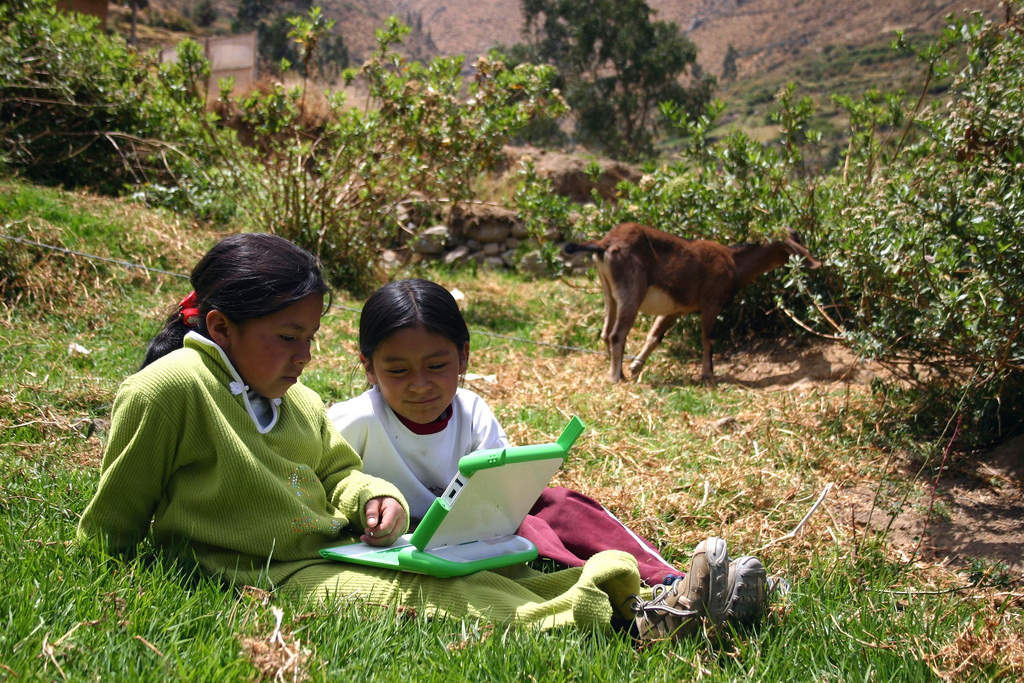
\includegraphics[height=17cm]{Bucolico-full.jpg}
    \end{tikzfigure}

    A Peruvian schoolchild finds no information in Wikipedia about
    their hometown, but can't contribute an article because they are
    using the wiki offline.

  }
  \column{0.33}
  \block{\myb{Tor!}}{%

    \begin{tikzfigure}
      
\includegraphics[height=15.65cm]{censored-nospeaking.eps}
    \end{tikzfigure}

    A user in a repressive regime can only safely access Wikipedia by
    using Tor, but in a catch-22 they then lose the ability to make
    contributions.

    \hfill(Read~more:~\url{http://andreaforte.net/ForteCSCW17-Anonymity.pdf})
  }
\end{columns}
\block{}{\centering\Huge\it Oh my!}
\begin{columns}
  \column{0.33}
  \newlength{\myfigwidth}
  \newlength{\mw}
  \setlength{\myfigwidth}{11cm}
  \setlength{\mw}{\colwidth}
  \addtolength{\mw}{-3cm}
  \addtolength{\mw}{-\myfigwidth}

  \block{\myb{Linear Edit Model}}{
    \begin{minipage}[b]{\mw}
    In today's MediaWiki, edits are only made to the most recent
    revision of an article.  Once a new revision is saved, any
    outstanding edits to the previous revision are not allowed to be
    saved.  The author needs to manually apply their edits to the
    most recent revision before their work can be saved.
    \end{minipage}\hfill\begin{minipage}[b]{\myfigwidth}
    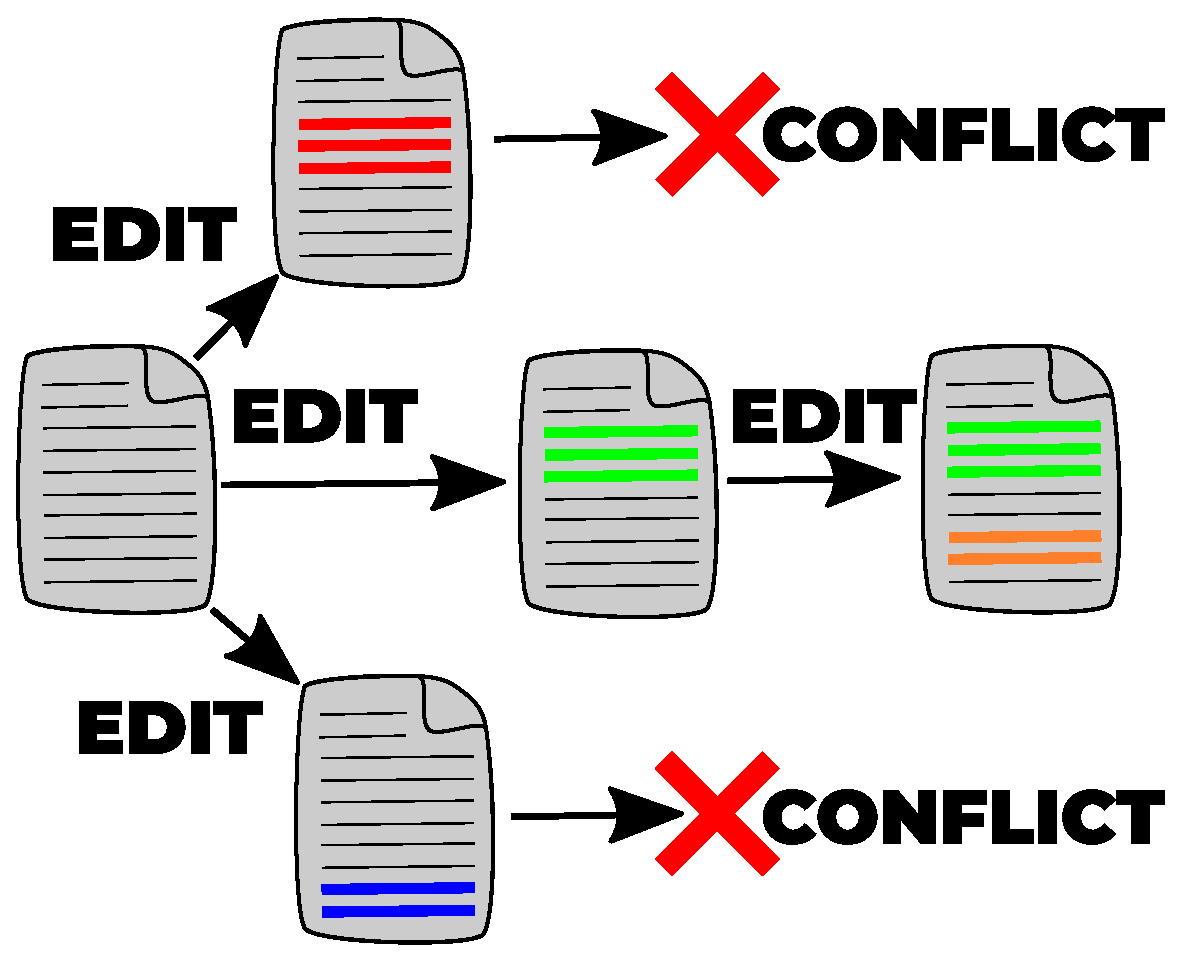
\includegraphics[height=7.6cm]{revision-no-fork.eps}
    \end{minipage}

    Although new tools attempt to make the revision of conflicts
    easier, they do not address the fundamental problem:
    edits can't be saved unless they apply to the most recent
    revision.
  }

  \block{\myb{Fork-Merge Edit Model}}{%
    \begin{minipage}[b]{\mw}
      With a fork-and-merge model, edits can always be saved, although
      only edits to the most recent revision are immediately merged
      and viewable.

      New users whose content isn't immediately merged find it
      preserved on their fork for revision and re-submission, reducing
      their sense of rejection and loss.

    \end{minipage}\hfill\begin{minipage}[b]{\myfigwidth}
        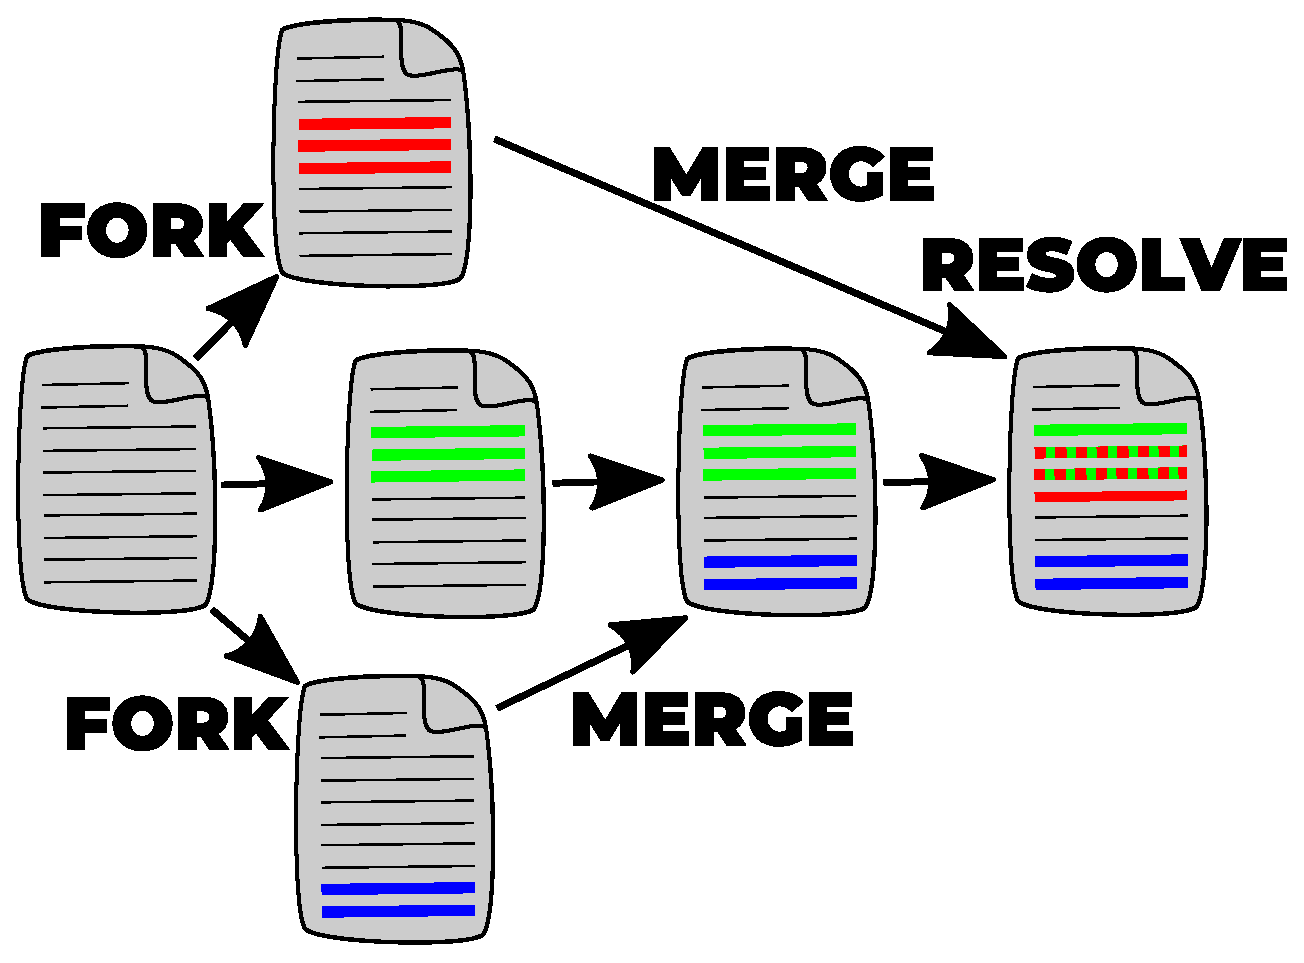
\includegraphics[height=7.6cm]{revision-fork.eps}
    \end{minipage}

      Online edits can be auto-saved to a fork, and conflict
      resolution safely deferred to a later session.
      Offline users who are forced to work on an out-of-date copy
      and those using the draft namespace can use the same
      resolution tools when their contributions are brought to merge.
      \hfill(More:~\url{https://phabricator.wikimedia.org/T113004})
    }

  \column{0.34}
  \setlength{\myfigwidth}{18cm}
  \setlength{\mw}{\colwidth}
  \addtolength{\mw}{-4cm}
  \addtolength{\mw}{-\myfigwidth}
  \block{\myb{Collaborative Edit Queues}}{%

    Although the vast majority of edits which can be applied without
    conflict or controversy would be merged immediately and
    automatically, forks could be created manually or (when conflicts
    arise) automatically.  Merging forks (and resolving any
    conflicts) can be done as a separate process, at a later time, and
    by anyone at all---not solely the original author of the edit!

    \begin{center}\textbf{Resolution can be done collaboratively
    by the community.}\end{center}

    \vspace{0.5cm}
  \begin{minipage}{\mw}
    Tools for merging conflicted edits can be built in a general
    fashion, not tightly tied to a particular edit tool.
    Forks are reachable from the main article, and volunteers can
    resolve/merge these forks.
  \end{minipage}\hfill\begin{minipage}{\myfigwidth}
    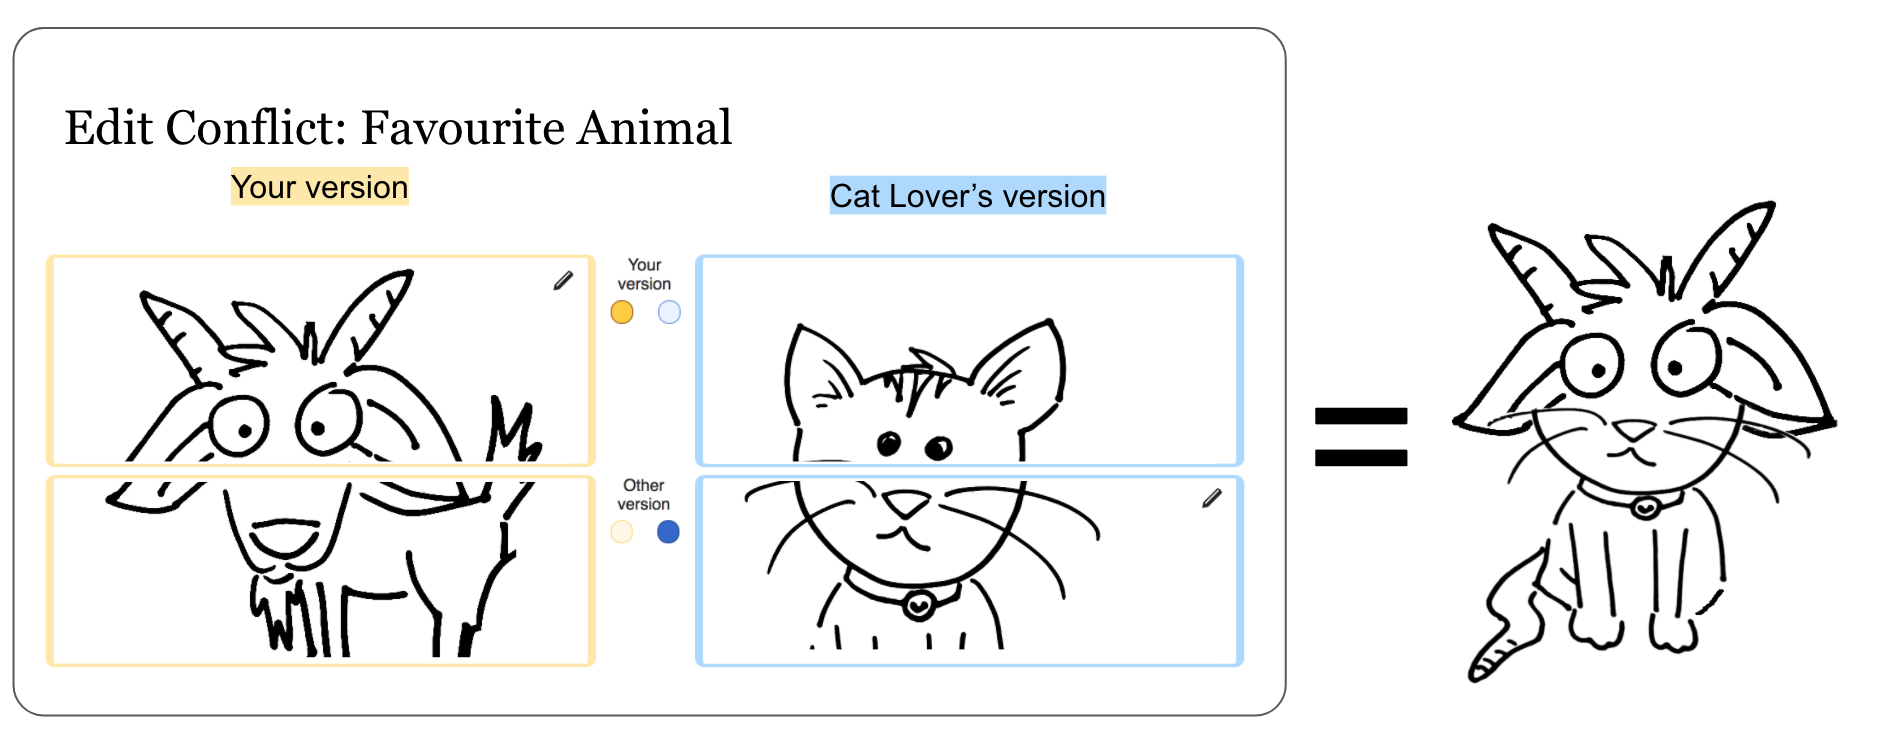
\includegraphics[height=6.5cm]{favourite-animal.png}
  \end{minipage}
    \vspace{0.75cm}

    \textbf{We have built a proof-of-concept
    for readers browsing via Tor, which lets them save their
    edits into a ``Suggestion Queue'' for later merge.}

    \begin{tikzfigure}
    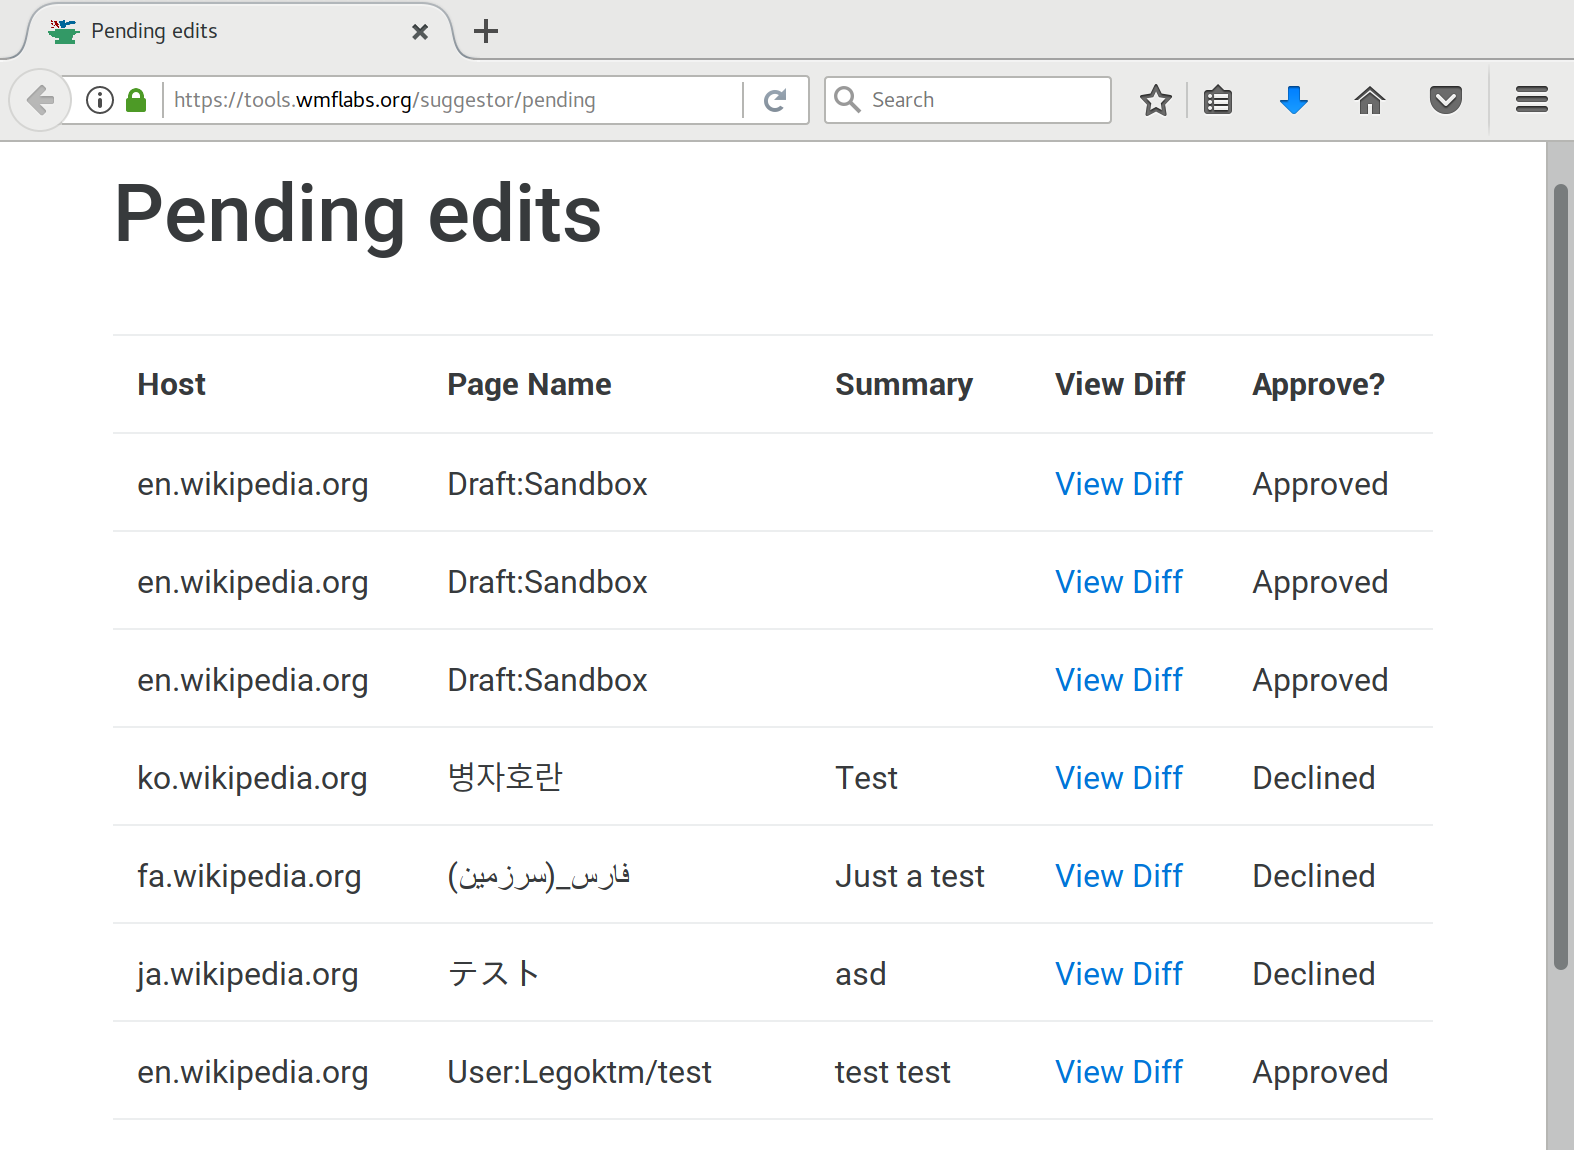
\includegraphics[height=9.1cm]{pending-edits.png}%
    \hspace{3cm}%
    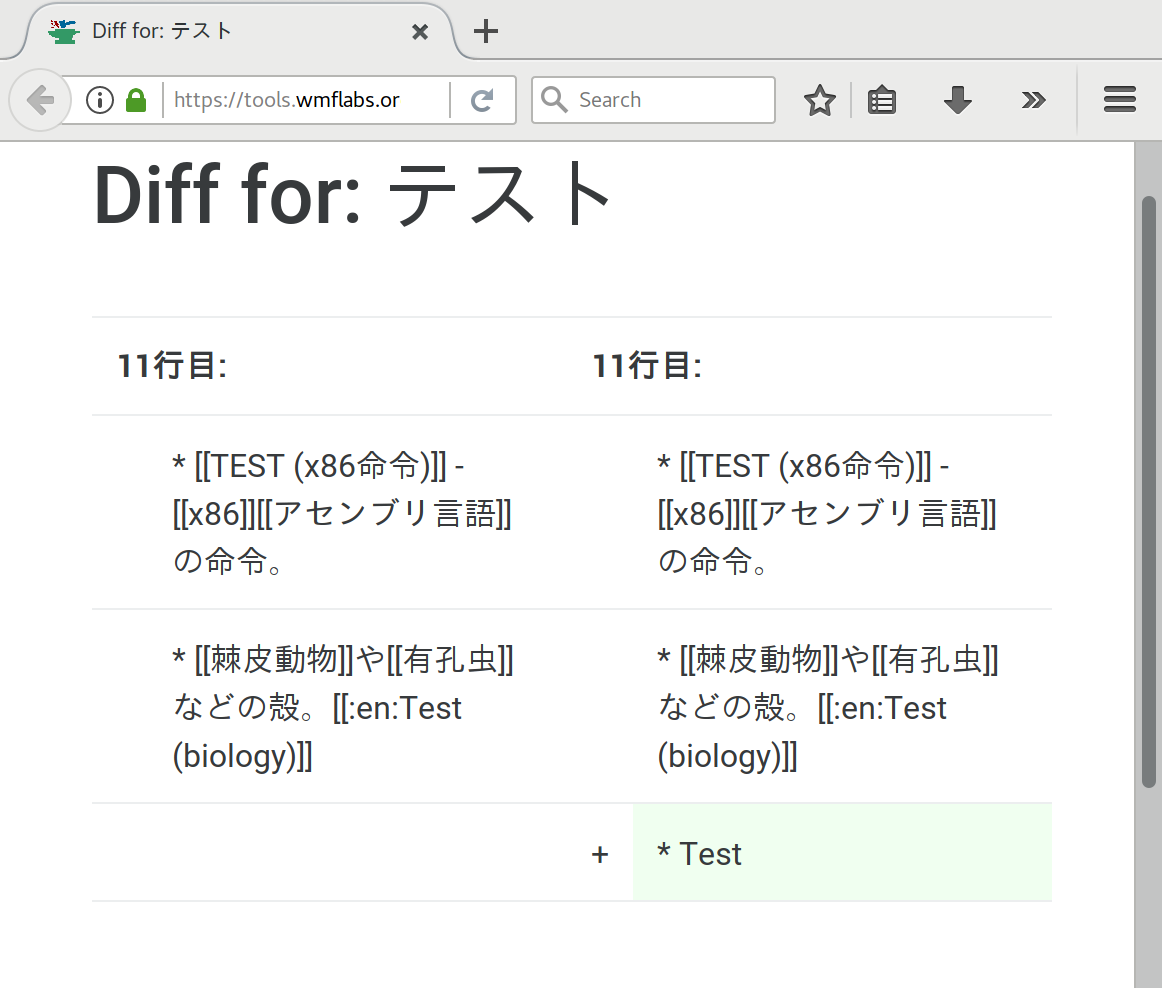
\includegraphics[height=9.1cm]{diff.png}%
    \\[10pt]
    {\small
      Collaborative queue for edits from
      Tor: \url{https://www.mediawiki.org/wiki/Suggestor}}
    \end{tikzfigure}
}
  \column{0.33}
  \block{\myb{Volunteer Communities}}{%

    Queues for merging contributions can be organized by volunteers
    according to interest group, and communities built.  Some examples:
    \begin{itemize}
    \item Unmerged edits by new editors
    \item Edits from Turkey/Syria/\ldots via Tor
    \item Edits from offline schoolkids in Peru/Ethiopia/\ldots
    \item Abandoned edit conflicts from articles on your watchlist
    \item Allies volunteering to be the public face of merges from
      harassed groups
    \end{itemize}

    We then can collect edits from more diverse and less-connected
    users and provide a friendlier first-edit experience to retain
    newcomers. Volunteer merge queues provide another means for those
    well-connected to aid those with difficulties in the spirit of
    \textit{ubuntu}. By increasing participation we can bridge the knowledge
    gap.

\begin{tikzfigure}
  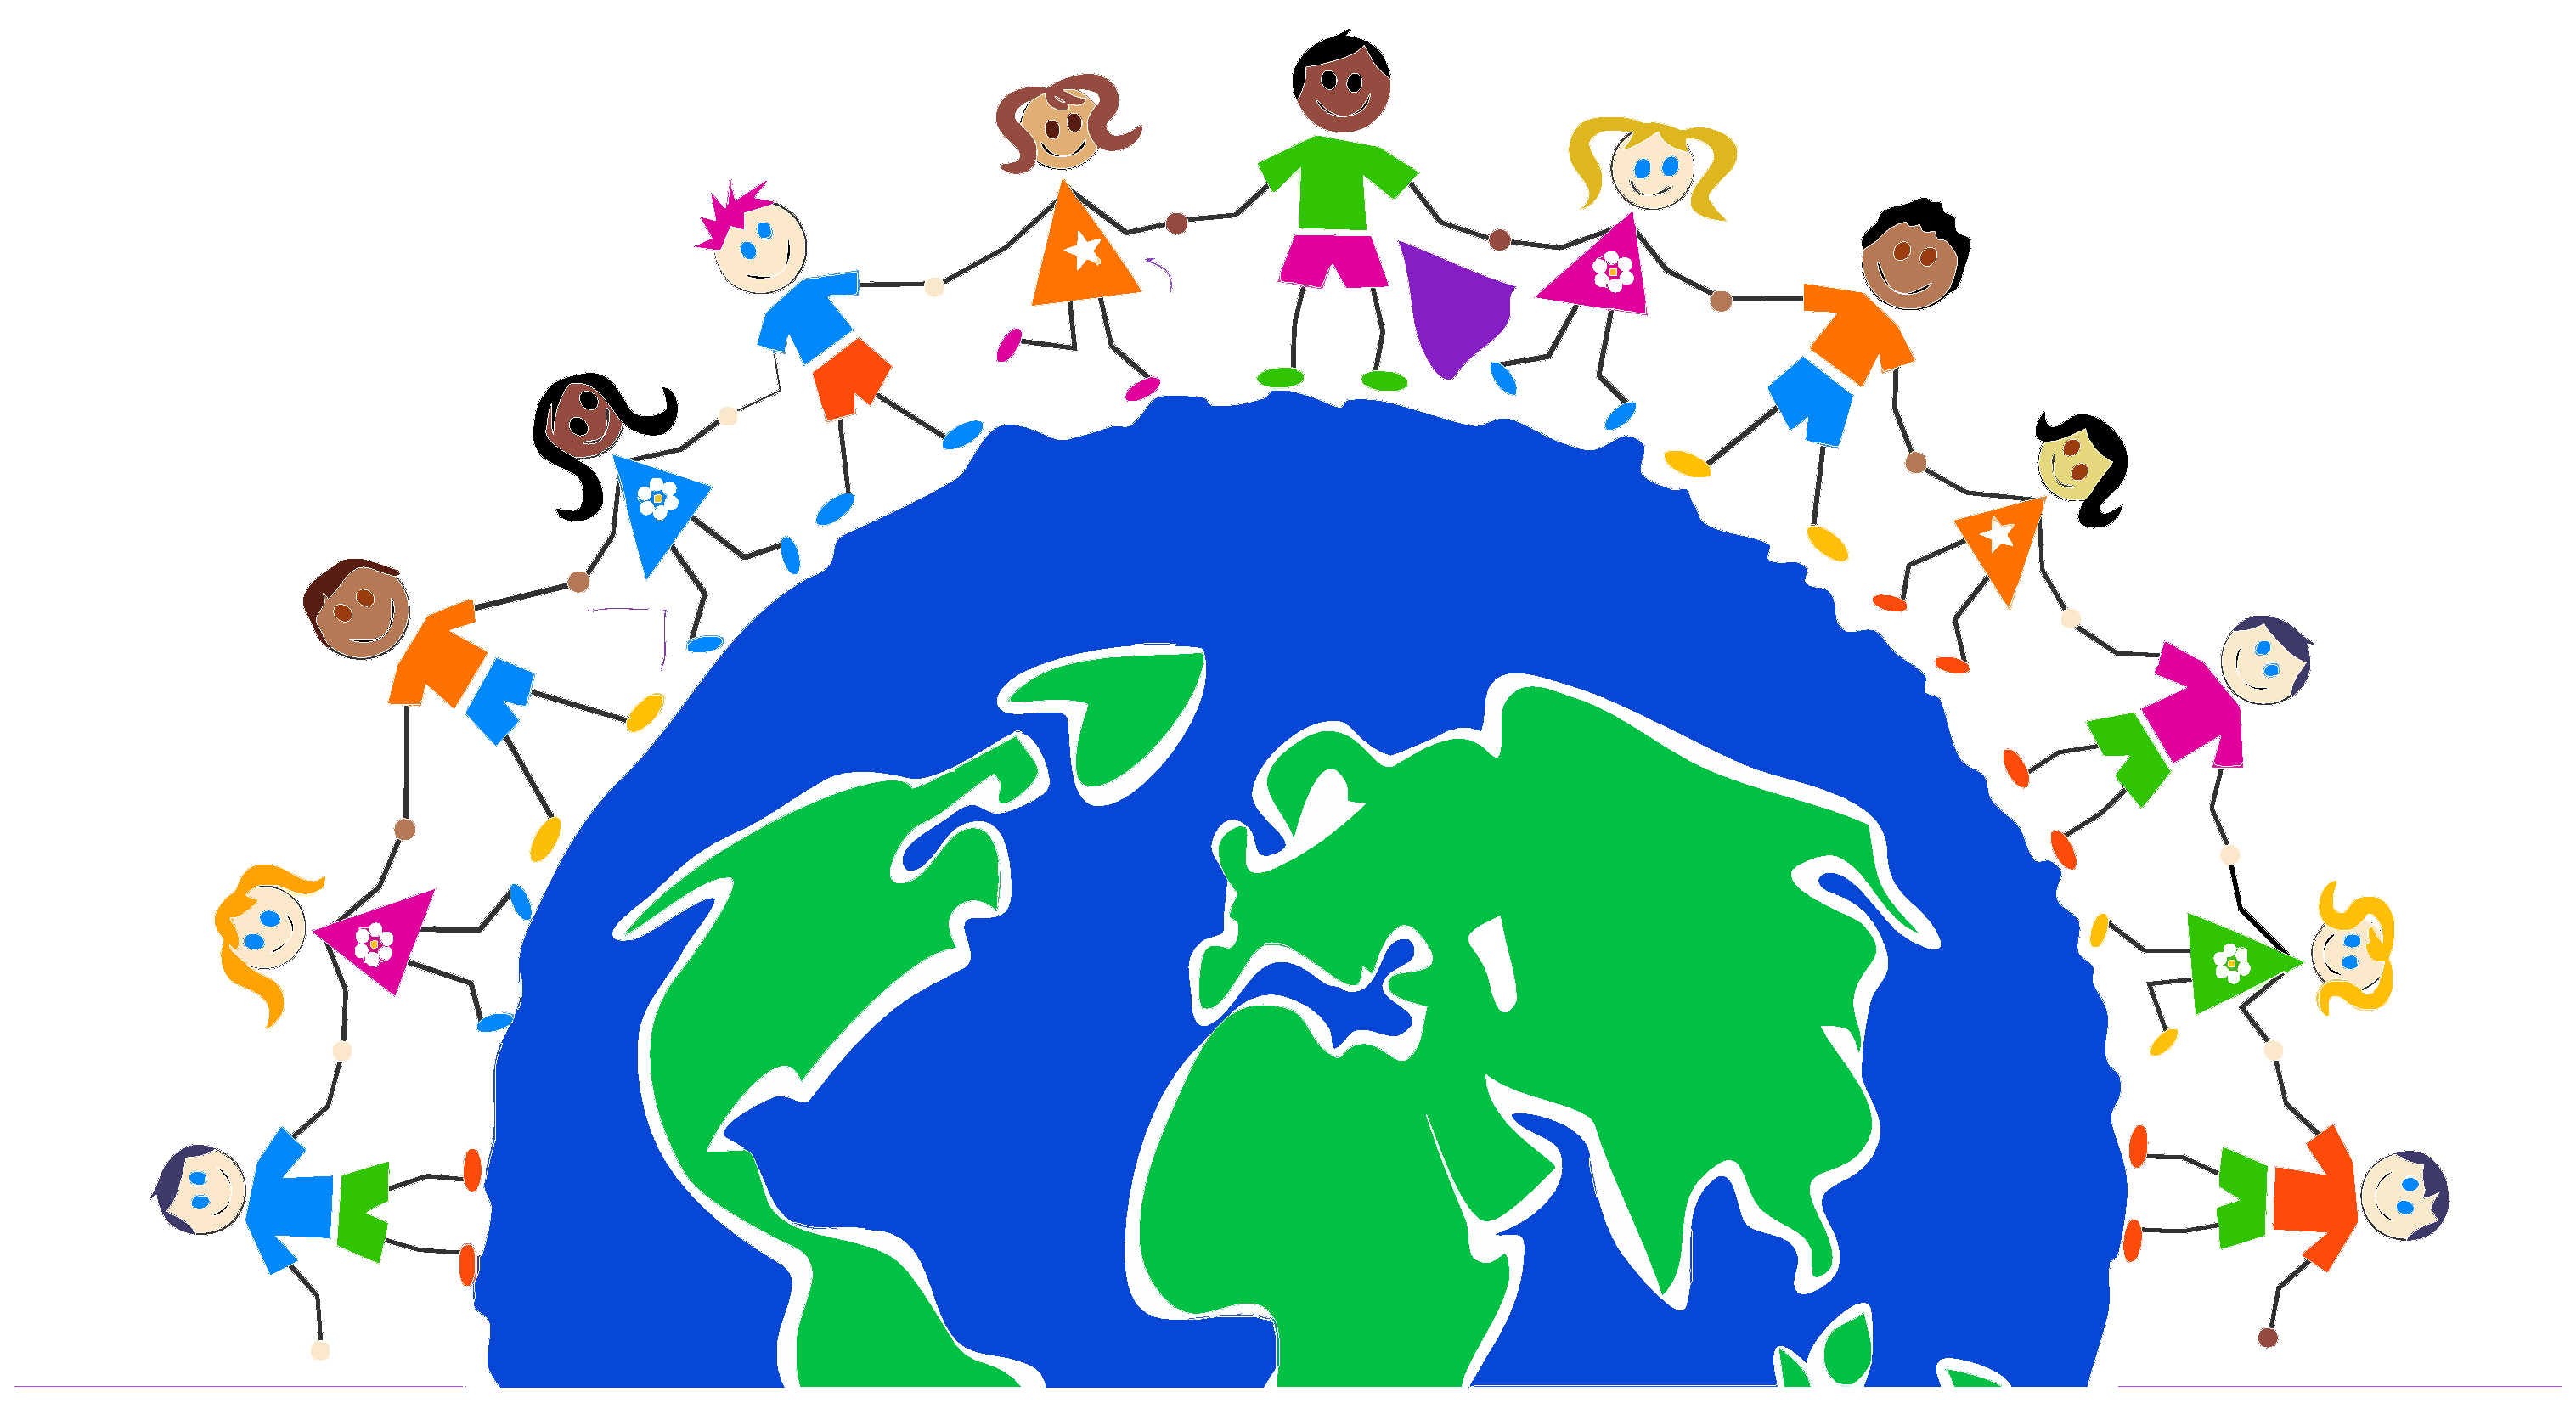
\includegraphics[height=14.45cm]{world-kids-nobg.eps}
\end{tikzfigure}
}
\end{columns}
\block{}{\centering\small
  Created with \LaTeX\ and TikZposter.
  \href{https://openclipart.org/detail/231887/conflict-silhouette}{conflict-silhouette}
    by \href{https://openclipart.org/user-detail/GDJ}{GDJ}
    / \href{http://creativecommons.org/publicdomain/zero/1.0/}{CC0};
  \url{http://wiki.laptop.org/go/File:Bucolico-full.jpg}
    by OLPC Peru
    / \href{https://creativecommons.org/licenses/by-sa/4.0/legalcode}{CC-SA};
  \href{https://openclipart.org/detail/296265/censored-no-speaking}{censored-no-speaking}
    by \href{https://openclipart.org/user-detail/j4p4n}{j4p4n}
    / \href{http://creativecommons.org/publicdomain/zero/1.0/}{CC0};
  \href{https://openclipart.org/detail/101161/page-or-document}{page-or-document}
    by \href{https://openclipart.org/user-detail/docguy}{docguy}
    / \href{http://creativecommons.org/publicdomain/zero/1.0/}{CC0};
  \href{https://commons.wikimedia.org/wiki/File:Paragraph-based_prototype_\%E2\%80\%93_rough_visualization_of_the_functionality.png}{Edit conflict}
    by \href{https://commons.wikimedia.org/wiki/User:Johanna_Strodt_(WMDE)}{Johanna\_Strodt\_(WMDE)}
    / \href{https://creativecommons.org/licenses/by-sa/4.0/legalcode}{CC-SA};
  \href{https://openclipart.org/detail/228325/world-kids}{world-kids}
    by \href{https://openclipart.org/user-detail/GDJ}{GDJ}
    / \href{http://creativecommons.org/publicdomain/zero/1.0/}{CC0}
    / Background removed.
}
\end{document}
